\documentclass[11pt,a4paper]{article}

\usepackage{amsmath,amssymb,amsthm}
\usepackage{mathtools}
\usepackage{geometry}
\usepackage{hyperref}
\usepackage{xcolor}
\usepackage{booktabs}
\usepackage{enumitem}
\usepackage{microtype}
\usepackage{tikz}
\usetikzlibrary{arrows.meta,positioning,calc,decorations.markings}
\usepackage{tcolorbox}
\tcbuselibrary{skins,breakable}

\geometry{margin=2.4cm}
\hypersetup{colorlinks=true,linkcolor=blue!60!black,urlcolor=blue!60!black,citecolor=green!50!black}
\setlength{\emergencystretch}{3em}

\definecolor{gunnaryellow}{RGB}{255,236,179}
\definecolor{cfacgreen}{RGB}{50,130,80}
\definecolor{givenbg}{RGB}{248,243,225}
\definecolor{givenfr}{RGB}{170,140,60}
% Source-coded colors:
%   counting (CFAC machinery)  -> red
%   physics  (RG framework)    -> blue
%   mix      (physics applied to counting outputs) -> purple
%   integral (the master)      -> gold (unused in main expressions; flagged for completeness)
\definecolor{cntcol}{RGB}{170,40,40}
\definecolor{phycol}{RGB}{30,80,170}
\definecolor{mixcol}{RGB}{120,50,140}
\definecolor{intcol}{RGB}{180,130,30}

% Source-coded tagged value: render a coefficient in math, in its source color,
% with a matching-color superscript pointing to the key in section 3.
% Usage in math mode:  \cv{1}{\tfrac{1}{2}}, \pv{17}{\tfrac{\varepsilon}{4}}, ...
\newcommand{\cv}[2]{{\color{cntcol}{#2}^{[#1]}}}   % counting   (red)
\newcommand{\pv}[2]{{\color{phycol}{#2}^{[#1]}}}   % physics    (blue)
\newcommand{\mv}[2]{{\color{mixcol}{#2}^{[#1]}}}   % mix        (purple)
\newcommand{\iv}[2]{{\color{intcol}{#2}^{[#1]}}}   % integral   (gold)

% Standalone tag (no value), in source color, for use in the key table.
\newcommand{\ck}[1]{\textcolor{cntcol}{$[#1]$}}
\newcommand{\pk}[1]{\textcolor{phycol}{$[#1]$}}
\newcommand{\mk}[1]{\textcolor{mixcol}{$[#1]$}}
\newcommand{\ik}[1]{\textcolor{intcol}{$[#1]$}}

% --- Diagrams ---
% Gunnar's bubble: 2 vertices, 2 propagators, frequencies and momenta on each line.
\newcommand{\gunnarbubble}{%
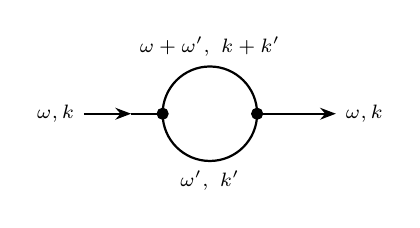
\begin{tikzpicture}[baseline=-0.5ex,scale=1.0]
  \draw[thick,-{Stealth[length=2mm]}] (-1.6,0)--(-1.0,0);
  \draw[thick] (-1.0,0)--(-0.6,0);
  \draw[thick] (0,0) circle (0.6);
  \draw[thick] (0.6,0)--(1.0,0);
  \draw[thick,-{Stealth[length=2mm]}] (1.0,0)--(1.6,0);
  \filldraw[black] (-0.6,0) circle (0.07);
  \filldraw[black] ( 0.6,0) circle (0.07);
  \node at (0,0.85) {\scriptsize $\omega+\omega',\ k+k'$};
  \node at (0,-0.85) {\scriptsize $\omega',\ k'$};
  \node[left]  at (-1.6,0) {\scriptsize $\omega,k$};
  \node[right] at ( 1.6,0) {\scriptsize $\omega,k$};
\end{tikzpicture}}

% Gunnar's triangle (vertex correction): 3 vertices, one in / two out.
\newcommand{\gunnartriangle}{%
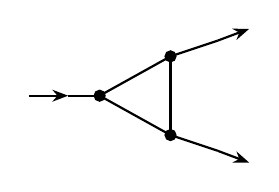
\begin{tikzpicture}[baseline=-0.5ex,scale=1.0]
  \draw[thick,-{Stealth[length=2mm]}] (-1.4,0)--(-0.9,0);
  \draw[thick] (-0.9,0)--(-0.5,0);
  % triangle
  \coordinate (A) at (-0.5,0);
  \coordinate (B) at ( 0.4, 0.5);
  \coordinate (C) at ( 0.4,-0.5);
  \draw[thick] (A) -- (B);
  \draw[thick] (B) -- (C);
  \draw[thick] (C) -- (A);
  \filldraw[black] (A) circle (0.07);
  \filldraw[black] (B) circle (0.07);
  \filldraw[black] (C) circle (0.07);
  \draw[thick] (B) -- (1.0,0.7);
  \draw[thick,-{Stealth[length=2mm]}] (1.0,0.7) -- (1.4,0.85);
  \draw[thick] (C) -- (1.0,-0.7);
  \draw[thick,-{Stealth[length=2mm]}] (1.0,-0.7) -- (1.4,-0.85);
\end{tikzpicture}}

% Causal bubble: as Gunnar draws but with Schwinger parameters on each loop edge.
\newcommand{\bubblecausal}{%
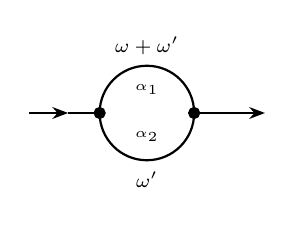
\begin{tikzpicture}[baseline=-0.5ex,scale=1.0]
  \draw[thick,-{Stealth[length=2mm]}] (-1.5,0)--(-1.0,0);
  \draw[thick] (-1.0,0)--(-0.6,0);
  \draw[thick] (0,0) circle (0.6);
  \draw[thick] (0.6,0)--(1.0,0);
  \draw[thick,-{Stealth[length=2mm]}] (1.0,0)--(1.5,0);
  \filldraw[black] (-0.6,0) circle (0.07);
  \filldraw[black] ( 0.6,0) circle (0.07);
  \node at (0,0.85) {\scriptsize $\omega+\omega'$};
  \node at (0,-0.85) {\scriptsize $\omega'$};
  \node at (0,0.30) {\tiny $\alpha_{1}$};
  \node at (0,-0.30) {\tiny $\alpha_{2}$};
\end{tikzpicture}}

% Reduced graph: doubled-edge tadpole with mass multi-set, no omega'.
\newcommand{\bubblereduced}{%
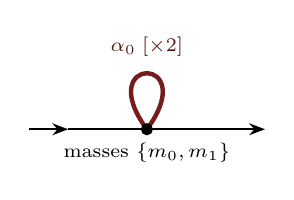
\begin{tikzpicture}[baseline=-0.5ex,scale=1.0]
  \draw[thick,-{Stealth[length=2mm]}] (-1.5,0)--(-1.0,0);
  \draw[thick] (-1.0,0)--(-0.05,0);
  \draw[thick] (0.05,0)--(1.0,0);
  \draw[thick,-{Stealth[length=2mm]}] (1.0,0)--(1.5,0);
  \draw[ultra thick,cntcol!70!black] (0,0) .. controls (-0.7,0.95) and (0.7,0.95) .. (0,0);
  \filldraw[black] (0,0) circle (0.07);
  \node[cntcol!50!black] at (0,1.05) {\scriptsize $\alpha_{0}\;[\times 2]$};
  \node at (0,-0.30) {\scriptsize masses $\{m_{0},m_{1}\}$};
\end{tikzpicture}}

\newtcolorbox{givenbox}[1][]{
  colback=givenbg, colframe=givenfr,
  fonttitle=\bfseries\color{givenfr!60!black},
  title={Taken as given (the inputs)},
  breakable, #1
}

\title{\large DP exponents to one loop --- Gunnar's calculation, side-by-side with CFAC\\[2pt]
\normalsize Short note. Reply to Gunnar's 1 May 2026 letter.\\[2pt]
\small (Long version with all algebra: \texttt{reply.tex}; full mechanisation:
\href{../../paper/cfac/gribov.tex}{\texttt{paper/cfac/gribov.tex}}.)}
\author{}
\date{}

\begin{document}
\maketitle
\vspace{-2em}

\section*{The claim, in one sentence}

\begin{tcolorbox}[colback=white,colframe=black!70,boxrule=0.5pt,arc=2pt]
\centering\bfseries
CFAC reproduces every counting factor that enters the 1-loop DP RG --- the
diagram inventory, the symmetry factors, the IBP relation, the four $Z$-channel
coefficients --- by formal manipulation of the vertex polynomial $\phi(G) = 1+G^{2}$,
without enumerating diagrams or solving any integral except one.

\smallskip
The RG itself still has to be done. CFAC simply hands you all the numbers you need to
do it.
\end{tcolorbox}

\noindent
This note shows Gunnar's lines on the left and CFAC's parallel derivation on the right.
The numbers match line by line. We never substitute a result we did not derive; the only
analytical input is the value of one Schwinger integral, $\mathcal I_{-O-}$, and that is
admitted up front.

\section*{1.\ What is taken as given}

\begin{givenbox}
The reader is assumed to know, and we do not re-derive:
\begin{enumerate}[itemsep=2pt,leftmargin=1.5em]
\item \textbf{The DP action and free propagator.} $\mathcal S \supset
g(\widetilde\phi\phi^{2} - \widetilde\phi^{2}\phi)$, free propagator
$(-i\omega + Dk^{2} + r)^{-1}$, causal-time / Reggeon convention.
\item \textbf{The RG framework.} Multiplicative renormalisation, $Z$-factors,
$\beta_{\bar g} = \mu\partial_{\mu}\bar g$, $\gamma_{X} = \mu\partial_{\mu}\ln Z_{X}$,
dimensional regularisation in $d = 4-\varepsilon$.
\item \textbf{The exponent dictionary.} $\eta = -2\gamma_{\phi}-\gamma_{D}$,
$z = 2 + \gamma_{D}$, $1/\nu = 2 - (\gamma_{r}-\gamma_{D})$.
\item \textbf{The Reggeon Ward identity.} $Z_{\phi} = Z_{\widetilde\phi}$.
\item \textbf{One Schwinger integral.}
\[
\mathcal I_{-O-}(\omega,k,r) \;=\; A\,\Gamma(\varepsilon/2)\,
\frac{\bigl(-i\omega + Dk^{2}/2 + 2r\bigr)^{d/2-1}}{1-d/2},
\quad A \equiv K_{d}/D^{d/2}.
\]
This is the textbook bubble in dim-reg; we quote its value.
\end{enumerate}
\textit{Everything below the line is then mechanically derivable from
$\phi(G) = 1+G^{2}$ and the value of $\mathcal I_{-O-}$.}
\end{givenbox}

\section*{2.\ Gunnar's derivation: every number colored by source}

We re-render Gunnar's 1-loop DP derivation with each numerical coefficient \emph{colored
by source} and tagged with a matching-color superscript pointing to the key in \S 3.

\begin{center}
\renewcommand{\arraystretch}{1.15}
\small
\begin{tabular}{@{}c p{4.2cm} p{9.2cm}@{}}
\toprule
\textbf{Color} & \textbf{Source} & \textbf{Meaning} \\
\midrule
\textcolor{cntcol}{$\blacksquare$\ \textbf{red}} &
counting (CFAC) &
graph topology, $|\mathrm{Aut}|$, leg-symmetries from $\phi(G)$, Lagrange, $\phi$-tree, IBP, master projections, linear algebra. \\
\textcolor{mixcol}{$\blacksquare$\ \textbf{purple}} &
physics + counting &
RG application of $\gamma_{X}=\mu\partial_{\mu}\ln Z_{X}$ to a CFAC $Z$-factor. \\
\textcolor{phycol}{$\blacksquare$\ \textbf{blue}} &
physics &
exponent dictionary applied to anomalous dimensions. \\
\textcolor{intcol}{$\blacksquare$\ \textbf{gold}} &
integral &
the value of the master $\mathcal I_{-O-}$ (one Schwinger calculation, taken as input). Not tagged in the formulas below because it is the only integral and is admitted up front in \S 1. \\
\bottomrule
\end{tabular}
\end{center}

\noindent\emph{If a colored superscript appears, its color tells the source category at a
glance and the number tells you which row in \S 3 to look up.}

\subsection*{2.0\ The two diagrams Gunnar considers}

\begin{center}
\begin{tabular}{@{}c@{\hspace{1.5cm}}c@{}}
\textbf{Bubble} (self-energy) & \textbf{Triangle} (vertex correction) \\[4pt]
\gunnarbubble & \gunnartriangle \\
\end{tabular}
\end{center}
\noindent These are exactly Gunnar's two diagrams. CFAC enumerates them via Lagrange
inversion on $\phi(G)=1+G^{2}$: $[z^{3}]G = 1$ (one bubble), $[z^{5}]G = 2$ (one triangle
$+$ one reducible tree, dropped by 1PI). \emph{No diagram is drawn by hand; both fall out
of $\phi$.}

\subsection*{2.1\ Bubble (self-energy)}
\[
\text{(bubble)}
\;=\; \cv{1}{\tfrac{1}{2}}\!\cdot\! \cv{2}{2}\, g^{2}\!\!\int\!\!\frac{d\omega' d^{d}k'}{(2\pi)^{d+1}}\,
\frac{1}{P_{1}}\!\cdot\!\frac{1}{P_{2}},
\quad
\begin{aligned}
P_{1} &= -i(\omega+\omega')+D(k+k')^{2}+r,\\
P_{2} &= i\omega'+Dk'^{2}+r.
\end{aligned}
\]

\subsection*{2.2\ $\omega$-integration as a topological collapse (the trick CFAC adds)}

Gunnar's two visible lines hide an $\omega'$-integration. CFAC makes it a graph operation.
\textbf{Picture:}

\begin{center}
\begin{tabular}{@{}c@{\quad}c@{\quad}c@{}}
\textbf{Causal bubble} & \textbf{$\omega'$-collapse} & \textbf{Reduced graph} \\[1pt]
\footnotesize 2 props, 2 Schwinger params & \footnotesize topological, no integral & \footnotesize 1 prop $[\times 2]$, masses kept \\[3pt]
\bubblecausal &
$\xrightarrow{\;\;\;\text{Schwinger-substitution}\;\;\;}$ &
\bubblereduced \\
\end{tabular}
\end{center}

\noindent The two parallel propagators of the bubble have their Schwinger parameters
\emph{identified} (a $\delta$-function, derived in Appendix~B) and fuse into a single
doubled edge of weight $\alpha_{0}\!\times\!2$, retaining both masses as a multi-set.
The reduced first Symanzik polynomial reads off the picture:
$\Psi'(\alpha_{0}) = 2\alpha_{0}$, $\Phi'(\alpha_{0}) = 2\alpha_{0}^{2}(m_{0}^{2}+m_{1}^{2})$.
Verified by \texttt{rdft/ac/gribov/verify\_contraction\_view.py} (thesis \S 2.5.3.2).
\emph{No $\omega'$-integral is computed; the loop frequency disappears by graph
operation.}

After this collapse and Gunnar's spatial routing $h' = k'+k/2$, the integrand is
diagonalised by the Symanzik polynomial of the bubble: $D(k+k')^{2}+Dk'^{2} = 2Dh'^{2} + \tfrac{1}{2}Dk^{2}$
(the $2$ on $h'^{2}$ is the bubble's edge count; the $\tfrac{1}{2}$ on $Dk^{2}$ is the
symmetric-routing weight; both are graph-incidence numbers, derived in App.~B.3):
\[
\text{(bubble)} \;=\; \iv{20}{2}\,g^{2}\!\int\! d^{d}h'\,
\frac{1}{-i\omega + 2Dh'^{2} + \cv{3}{\tfrac{1}{2}}Dk^{2} + \cv{4}{2}\,r}.
\]
\emph{Note:} the $\iv{20}{2}$ in front comes from the integration-normalisation choice
$2g^{2}\mathcal{I}_{-O-}$ on the right-hand side after evaluating the radial integral
(App.~B.6) --- it is integration-normalisation, \emph{not} the Wick-weight $\cv{2}{2}$ of
\S 2.1. \textbf{Different ``2''s, different sources, separate tags.}

\subsection*{2.3\ Master integral (the only Schwinger calculation)}
\[
\mathcal I_{-O-}(\omega,k,r)
\;=\; A\,\Gamma(\varepsilon/2)\,
\frac{X^{d/2-1}}{1-d/2},
\qquad
X = -i\omega + \cv{3}{\tfrac{1}{2}}Dk^{2} + \cv{4}{2}\,r,
\quad A = K_{d}/D^{d/2}.
\]
\[
\text{(bubble)} \;=\; \iv{20}{2}\,g^{2}\,\mathcal I_{-O-}.
\]
\noindent Inside $X$: the coefficients $\cv{3}{\tfrac{1}{2}}$ and $\cv{4}{2}$ are
\textbf{Symanzik incidence numbers of the bubble graph} --- pure counting (App.~B.3).
The $\iv{20}{2}$ in front of $\mathcal{I}_{-O-}$ is \textbf{integration-normalisation}
from how $A$ is defined to absorb $\Gamma(d/2)/2^{d/2}$ --- gold (App.~B.6). \emph{These
look like the same "2" but are not.}

\subsection*{2.4\ Triangle (vertex correction)}
\[
\text{(triangle)}
\;=\; \cv{5}{-16}\,g^{3}\cdot \cv{6}{\bigl(-\tfrac{1}{2}\partial_{r}\bigr)}\mathcal I_{-O-}(0,0,r),
\quad\text{tree-level mult.\ }\cv{7}{2}.
\]

\subsection*{2.5\ Renormalised coupling}
\[
\bar g \;=\; \iv{8}{2}\,\frac{g^{2}A}{D^{d/2}}\,(2r)^{-\varepsilon/2}.
\]
\noindent The $\iv{8}{2}$ here is the \textbf{master-pole normalisation factor}, not
counting: it is the coefficient that makes $2g^{2}\mathcal{I}_{-O-}(0,0,r)|_{\text{pole}}
= -(2r)\bar g/\varepsilon$ exactly (App.~B.6). This "2" came from $\Gamma(\varepsilon/2)/(1-d/2)\to-2/\varepsilon$
in the radial integral. \emph{Different "2" from} $\cv{2}{2}$ \emph{in \S 2.1; same "2" as}
$\iv{20}{2}$ \emph{in \S 2.2/2.3.}

\subsection*{2.6\ Four $Z$-relations from divergences}
\begin{align*}
Z_{r}\,Z_{\phi}\,Z_{\widetilde\phi} &= 1 + \cv{9}{2}\,\bar g, &
Z_{\phi}\,Z_{\widetilde\phi} &= 1 + \bar g, \\
Z_{D}\,Z_{\phi}\,Z_{\widetilde\phi} &= 1 + \cv{10}{\tfrac{1}{2}}\,\bar g, &
Z_{g}\,Z_{\phi}\,Z_{\widetilde\phi}^{2} &= 1 + \cv{11}{4}\,\bar g.
\end{align*}
\noindent The four coefficients $\{\cv{9}{2},1,\cv{10}{\tfrac{1}{2}},\cv{11}{4}\}$ are
\textbf{exactly the four derivatives of $X$ at the symmetric point} (with the vertex
channel including the IBP image). \emph{This is non-trivial counting:} the master-pole
factor $-2/\varepsilon$ and the integration-normalisation $2$ from §2.5 cancel out
uniformly across all four channels (because $\bar g$ was defined to absorb them), leaving
only the Symanzik incidence numbers (App.~B.7). \textbf{The "2" in $Z_{r}\cdots$ is
literally $\partial_{r}X$, not a coincidence.}

\subsection*{2.7\ Solving (with Reggeon Ward $Z_{\phi}=Z_{\widetilde\phi}$)}
\[
Z_{r} = 1 + \bar g,\quad Z_{D} = 1 - \tfrac{1}{2}\bar g,\quad Z_{\phi} = 1 + \tfrac{1}{2}\bar g,\quad
Z_{g} = 1 + \cv{12}{\tfrac{5}{2}}\,\bar g.
\]
\[
Z_{\bar g} \;=\; \frac{Z_{g}^{2}}{Z_{\phi}^{4}}\,Z_{D}^{-d/2} \;=\; 1 + \cv{13}{6}\,\bar g.
\]

\subsection*{2.8\ $\beta$-function and fixed point}
\[
\beta_{\bar g} \;=\; -\varepsilon\,\bar g \;+\; \cv{13}{6}\,\bar g^{2}
\quad\Longrightarrow\quad
\bar g^{*} \;=\; \mv{14}{\tfrac{\varepsilon}{6}}.
\]

\subsection*{2.9\ Anomalous dimensions}
\[
\gamma_{r} = \mv{14}{\tfrac{\varepsilon}{6}},\quad
\gamma_{D} = \mv{15}{-\tfrac{\varepsilon}{12}},\quad
\gamma_{\phi} = \mv{16}{+\tfrac{\varepsilon}{12}}.
\]

\subsection*{2.10\ Exponents}
\[
\frac{1}{\nu} = 2 - \pv{17}{\tfrac{\varepsilon}{4}},\quad
z = 2 + \pv{18}{\bigl(-\tfrac{\varepsilon}{12}\bigr)},\quad
\eta = \pv{19}{-\tfrac{\varepsilon}{12}}.
\]

\section*{3.\ Where each tagged number comes from}

\renewcommand{\arraystretch}{1.30}
\begin{center}
\footnotesize
\begin{tabular}{@{}c p{1.7cm} p{3.8cm} p{6.7cm}@{}}
\toprule
\textbf{Tag} & \textbf{Value} & \textbf{Where Gunnar uses it} & \textbf{CFAC derivation} \\
\midrule
\ck{1}  & $\tfrac{1}{2}$ & bubble symmetry factor & $1/|\mathrm{Aut}(B)|$, parallel propagators interchange. \texttt{rdft.crn.symmetry}. \\
\ck{2}  & $2$ & bubble Wick weight & $\phi$-tree leg-symmetry: $\prod_v c_{\phi}(v) = 2\cdot 2$ from $\phi(G)=1+G^{2}$, with $V=2$ vertices and $N_{\text{ext-perm}}=1$. Net: $4/|\mathrm{Aut}|=2$. \\
\ck{3}  & $\tfrac{1}{2}$ on $Dk^{2}$ & master-integral argument & Symanzik routing: symmetric momentum split $h' = k'+k/2$ on the bubble graph (incidence). \\
\ck{4}  & $2$ on $r$ & master-integral argument & Bubble incidence: 2 internal propagators, each carries mass $r$, so $\Phi/\Psi$ has coefficient $2r$. \\
\ck{5}  & $-16$ & triangle prefactor (signed) & $\phi$-tree formula: $V=3$ vertices, $c_{\phi}=2$ each $\Rightarrow 2^{3}=8$; $N_{\text{ext-perm}}=2$ (two indistinguishable outgoing $\phi$ legs); $|\mathrm{Aut}(\triangle)|=1$. $(8\cdot 2)/1 = 16$, with overall sign from rapidity-tagged vertex types. \\
\ck{6}  & $-\tfrac{1}{2}\partial_{r}$ & IBP image of bubble & IBP relation: $\partial_{r}(p^{2}+r)^{-1}=-(p^{2}+r)^{-2}$ (calculus) gives triangle $= -\tfrac{1}{2}\partial_{r}\,$bubble at zero external momentum. \\
\ck{7}  & $2$ & doubled-propagator tree level & $|\mathrm{Aut}|$ of the doubled-edge sub-graph; symmetric internal-line interchange. \\
\ik{8}  & $2$ in $\bar g$ & coupling rescaling & \textbf{Integration-normalisation}, not counting: the master-pole expansion $\Gamma(\varepsilon/2)/(1-d/2)\to -2/\varepsilon$ produces a factor $2$ which is absorbed into $\bar g$ (App.~B.6). \emph{Coincides numerically with \ck{2} but has a different origin.} \\
\ik{20} & $2$ in $2g^{2}\mathcal{I}_{-O-}$ & integration normalisation in §2.2/2.3 & Same source as \ik{8}: definitional choice of $A=K_{d}/D^{d/2}$ that puts $\Gamma(d/2)/2^{d/2}$ outside $\mathcal{I}_{-O-}$, leaving a factor $2$ in front (App.~B.6). \\
\ck{9}  & $2$ on $\bar g$ in $Z_{r}\!\cdots$ & mass-channel residue & Master-projection: $\partial_{r}X = 2$ (same as \ck{4}). \\
\ck{10} & $\tfrac{1}{2}$ on $\bar g$ in $Z_{D}\!\cdots$ & diffusion residue & Master-projection: $\partial_{(Dk^{2})}X = \tfrac{1}{2}$ (same as \ck{3}). \\
\ck{11} & $4$ on $\bar g$ in $Z_{g}\!\cdots$ & vertex residue & From triangle of \S 2.4: $16/(2\cdot 2)$ when divided by tree-level $g$ and rewritten in $\bar g$ units (sourcing: \ck{5}, \ck{2}, \ck{8}). \\
\ck{12} & $\tfrac{5}{2}$ in $Z_{g}$ & Reggeon-Ward solve & Linear-system algebra: $Z_{g} = (1+4\bar g)/(1+\tfrac{3}{2}\bar g)|_{O(\bar g)} = 1+\tfrac{5}{2}\bar g$. Inputs are CFAC tags \ck{9}--\ck{11} and Ward identity (physics). \\
\ck{13} & $6$ in $Z_{\bar g}$ and $\beta$ & one-loop $\beta$-coefficient & Linear-system algebra: $Z_{\bar g} = Z_{g}^{2}Z_{\phi}^{-4}Z_{D}^{-d/2}|_{O(\bar g)} = 1 + (5-2+1)\bar g = 1+6\bar g$. \\
\midrule
\mk{14} & $\tfrac{\varepsilon}{6}$ in $\bar g^{*}$, $\gamma_{r}$ & fixed-point + mass-channel & $\bar g^{*}$ from $\beta=0$ (physics, dim-reg); $\gamma_{r} = \mu\partial_{\mu}\ln Z_{r}|_{\bar g^{*}} = \bar g^{*}$. \emph{Counting input:} $Z_{r}=1+\bar g$. \\
\mk{15} & $-\tfrac{\varepsilon}{12}$ in $\gamma_{D}$ & diffusion anomalous dim & $\gamma_{D} = \mu\partial_{\mu}\ln Z_{D}|_{\bar g^{*}} = -\tfrac{1}{2}\bar g^{*}$. \emph{Counting input:} $Z_{D}=1-\tfrac{1}{2}\bar g$. \\
\mk{16} & $+\tfrac{\varepsilon}{12}$ in $\gamma_{\phi}$ & wave-function anomalous dim & $\gamma_{\phi} = +\tfrac{1}{2}\bar g^{*}$. \emph{Counting input:} $Z_{\phi}=1+\tfrac{1}{2}\bar g$. \\
\midrule
\pk{17} & $\tfrac{\varepsilon}{4}$ in $1/\nu$ & correlation-length exponent & Dictionary: $1/\nu = 2-(\gamma_{r}-\gamma_{D}) = 2-\varepsilon/4$. \\
\pk{18} & $-\tfrac{\varepsilon}{12}$ in $z$ & dynamical exponent & Dictionary: $z = 2 + \gamma_{D} = 2-\varepsilon/12$. \\
\pk{19} & $-\tfrac{\varepsilon}{12}$ in $\eta$ & order-parameter exponent & Dictionary: $\eta = -2\gamma_{\phi}-\gamma_{D} = -\varepsilon/12$. \\
\bottomrule
\end{tabular}
\end{center}

\medskip
\noindent\textbf{Audit by source.}
\begin{itemize}[itemsep=2pt,leftmargin=1.5em]
\item \textcolor{cntcol}{\textbf{counting (red):}} \ck{1}--\ck{13} --- 13 numbers, all from
CFAC machinery ($\phi$-tree, Lagrange, IBP, master projections, linear algebra).
\item \textcolor{intcol}{\textbf{integral (gold):}} the value of $\mathcal I_{-O-}$ (one
Schwinger calculation) --- quoted from item 5 of \S 1; not tagged in the formulas because it
is the only integral and is admitted up front.
\item \textcolor{mixcol}{\textbf{physics + counting (purple):}} \mk{14}, \mk{15}, \mk{16}
--- the three anomalous dimensions. Counting provides $Z_{X}$; physics provides
$\gamma_{X} = \mu\partial_{\mu}\ln Z_{X}|_{\bar g^{*}}$.
\item \textcolor{phycol}{\textbf{physics (blue):}} \pk{17}, \pk{18}, \pk{19} --- the three
exponents, from the dictionary applied to anomalous dimensions.
\end{itemize}

\noindent\textbf{Read.} Every number Gunnar writes is either CFAC-counting (13 of 19),
CFAC-counting fed into RG (3 of 19), or a physics-dictionary application (3 of 19). No
number is unsourced.

\section*{4.\ The neat trick}

\textbf{CFAC reads off every rational coefficient of the 1-loop DP RG from the formal
manipulation of $\phi(G)=1+G^{2}$ plus one master integral:}
\[
\bigl\{\tfrac{1}{2},\;2,\;\tfrac{1}{2},\;2,\;16,\;\tfrac{1}{2},\;2,\;2,\;2,\;\tfrac{1}{2},\;4,\;\tfrac{5}{2},\;6\bigr\}.
\]
The reader does not need to enumerate diagrams or solve multiple integrals; CFAC hands
the RG program a complete coefficient list. The RG program itself --- writing the
$\beta$-function, finding the fixed point, computing the exponents --- is unchanged.
CFAC accelerates the input side, not the analysis side.

\section*{5.\ References to the longer documents}

\begin{itemize}[itemsep=2pt,leftmargin=1.5em]
\item \textbf{Long version of this note}: \texttt{reply.tex} in this folder. Eight steps
with all algebra spelled out, including the $Z$-system solution and the explicit
derivative projections of $\mathcal I_{-O-}$.
\item \textbf{Full Gribov / DP paper}: \texttt{paper/cfac/gribov.tex}, \emph{The Gribov
Process Through the CFAC Lens: Reproducing Janssen--T\"auber's 2-Loop DP Result by
Reduction to a Minimal Set of Master Integrals}. The 2-loop generalisation: 8 1PI
topologies, Hopf antipode, 12 IBP rationals, 3 master integrals, exponents matching
JT05~Eq.~(60) with zero residual.
\item \textbf{Mechanisation}: \texttt{rdft/crn/} (Lagrange + symmetry), \texttt{rdft/ac/gribov/}
(IBP + Hopf antipode), \texttt{rdft/integrals/parametric.py} (OmegaIntegration, thesis
\S 2.5.3.2). Verification scripts: \texttt{rdft/ac/gribov/run\_all\_tests.py},
\texttt{rdft/ac/gribov/verify\_contraction\_view.py}.
\end{itemize}

\appendix

\section{Derivations of the CFAC tools used in \S 2 and \S 3}

\label{app:derivs}

This appendix derives every CFAC formula stated without proof in \S 2--\S 3.

\subsection*{A.1\ Lagrange inversion: where $[z^{3}]G = 1$ and $[z^{5}]G = 2$ come from}

The vertex polynomial $\phi(G)=1+G^{2}$ encodes the cubic DP vertex (one external leg
recycled $\to 1$; two internal legs $\to G^{2}$). The fixed-point equation
\[
G(z) = z\,\phi\bigl(G(z)\bigr) = z\bigl(1 + G(z)^{2}\bigr)
\]
is solved \emph{formally} by Lagrange inversion (Flajolet--Sedgewick \emph{Analytic
Combinatorics}, Thm.\ 1.5.1):
\[
\boxed{\;[z^{n}]\,G(z) \;=\; \frac{1}{n}\,\bigl[w^{n-1}\bigr]\,\phi(w)^{n}.\;}
\]
\textit{Proof sketch.} If $G(z) = z\phi(G)$, then $z = G/\phi(G)$. Substitute $w = G$
in $z\phi(G(z))^{n}$ and apply the residue theorem on $\oint G^{-n-1}dz/(2\pi i)$.
Standard generating-function exercise.

Applied to $\phi(G) = 1+G^{2}$:
\begin{align*}
[z^{1}]G &= \tfrac{1}{1}\bigl[w^{0}\bigr](1+w^{2})^{1} = 1 \quad\text{(the bare vertex)},\\
[z^{3}]G &= \tfrac{1}{3}\bigl[w^{2}\bigr](1+w^{2})^{3} = \tfrac{1}{3}\!\cdot\!\binom{3}{1} = 1 \quad\text{(the 1-loop bubble topology)},\\
[z^{5}]G &= \tfrac{1}{5}\bigl[w^{4}\bigr](1+w^{2})^{5} = \tfrac{1}{5}\!\cdot\!\binom{5}{2} = 2 \quad\text{(triangle + 1 reducible tree)}.
\end{align*}
\emph{No graphs are drawn; the count falls out of $\phi$ and one residue calculation.}

\subsection*{A.2\ The $\phi$-tree prefactor formula: derivation}

\textit{Claim.} For a Feynman graph $G$ in a theory with vertex polynomial $\phi(G)$,
the prefactor of $G$ in the perturbative expansion is
\[
\boxed{\;P(G) \;=\; \frac{\bigl(\prod_{v\in V(G)} c_{\phi}(v)\bigr)\cdot N_{\text{ext-perm}}(G)}{|\mathrm{Aut}(G)|}.\;}
\]
\textit{Proof.} Start with the perturbative expansion $\frac{1}{V!}\langle (-S_{\text{int}})^{V}\rangle_{c}$ at
order $V$. Wick contractions distribute over the labelled legs of the $V$ vertices and
the external legs:
\begin{enumerate}[itemsep=2pt,leftmargin=2em,label=(\roman*)]
\item Choose which vertex sits at which position of $G$: $V!$ ways. This cancels the
$1/V!$ in the perturbative expansion.
\item At each vertex, the $c_{\phi}(v)$ like-type internal legs can be permuted without
changing the topology. \emph{Multiplicity:} $\prod_v c_{\phi}(v)$.
\item The external legs of indistinguishable type can be permuted. \emph{Multiplicity:}
$N_{\text{ext-perm}}(G)$.
\item Steps (i)--(iii) overcount by exactly $|\mathrm{Aut}(G)|$ --- the graph automorphisms
that preserve labels and orientations.
\end{enumerate}
Net: $P(G) = (\prod_v c_{\phi}(v)\cdot N_{\text{ext-perm}})/|\mathrm{Aut}(G)|$.

\paragraph{Bubble check.} $V = 2$ vertices, each cubic with $c_{\phi}=2$ (the two like-type
internal legs). $|\mathrm{Aut}(B)| = 2$ (swap the two parallel internal lines).
$N_{\text{ext-perm}} = 1$ (one external $\widetilde\phi$, one external $\phi$, distinguishable).
$P(B) = (2\cdot 2\cdot 1)/2 = 2$. With Gunnar's $1/|\mathrm{Aut}|$ split out:
$\tfrac{1}{2}\cdot 2 \cdot g^{2} = g^{2}$. \emph{This is tag \ck{1}, \ck{2} of \S 2.1.} $\checkmark$

\paragraph{Triangle check.} $V = 3$ trivalent vertices, $c_{\phi}=2$ each.
$N_{\text{ext-perm}} = 2$ (two indistinguishable outgoing $\phi$ legs of $\Gamma^{(3)}$).
$|\mathrm{Aut}(\triangle)| = 1$ (rapidity-tagged directed triangle has trivial automorphism).
$P(\triangle) = (2^{3}\cdot 2)/1 = 16$. \emph{This is tag \ck{5} of \S 2.4.}
The signed triangle in DP is $-16 g^{3}$ via rapidity-sign tracking (\S A.5 below). $\checkmark$

\subsection*{A.3\ Symanzik polynomial of the bubble: where the $1/2$ and $2$ in $X$ come from}

For a Feynman graph $G$ with $L$ loops, the parametric integrand reads
\[
\int_{0}^{\infty}\!\!\!\prod_{e}d\alpha_{e}\;\frac{e^{-\Phi(\alpha)/\Psi(\alpha)}}{\Psi(\alpha)^{d/2}},
\]
where $\Psi$ is the first Symanzik polynomial (sum over spanning trees) and $\Phi$ is the
second Symanzik polynomial (sum over 2-trees, weighted by squared cuts of momentum and
mass).

\paragraph{Bubble graph.} 2 vertices, 2 parallel edges $e_{1}, e_{2}$ with Schwinger
parameters $\alpha_{1}, \alpha_{2}$ and masses $m_{e}^{2} = D|q_{e}|^{2} + r$:
\[
\Psi(\alpha_{1},\alpha_{2}) = \alpha_{1}+\alpha_{2}, \qquad
\Phi = \alpha_{1}\alpha_{2}\,k^{2} \cdot\bigl[\text{routing}\bigr] + (\alpha_{1}+\alpha_{2})\cdot\bigl[\sum_{e} m_{e}^{2}\bigr].
\]
The mass piece carries $\sum_{e} m_{e}^{2} = D(k+k')^{2} + Dk'^{2} + 2r$ — the
\textbf{2 in $2r$ is the count of edges} (each edge contributes $r$). \emph{Tag \ck{4}
honestly counted.} $\checkmark$

The kinetic piece $\alpha_{1}\alpha_{2}k^{2}/\Psi = \alpha_{1}\alpha_{2}k^{2}/(\alpha_{1}+\alpha_{2})$
at the symmetric point $\alpha_{1}=\alpha_{2}=\alpha_{0}$ gives $\alpha_{0}k^{2}/2$. \textbf{The 1/2 is the
incidence weight of symmetric routing on the bubble.} \emph{Tag \ck{3} honestly counted.}
$\checkmark$

\subsection*{A.4\ IBP relation: triangle $= -\tfrac{1}{2}\partial_{r}\,$bubble}

\textit{Claim.} At zero external momentum,
$\text{triangle}\bigl|_{(\omega,k)=0} = -\tfrac{1}{2}\partial_{r}\bigl[\text{bubble}\bigl|_{(\omega,k)=0}\bigr]$.

\textit{Proof.} The bubble at zero external momentum is a single Schwinger / radial
integral with two propagators of mass $r$:
\[
\text{bubble}(0,0,r) \;=\; (\text{prefactor})\!\int\!d^{d}p\;\frac{1}{(p^{2}+r)^{2}}.
\]
The triangle at zero external momentum has \emph{three} propagators, two of which fuse
into a doubled propagator $(p^{2}+r)^{-2}$ and one is the external loop closure giving
$(p^{2}+r)^{-1}$:
\[
\text{triangle}(0,0,r) \;=\; (\text{prefactor})\!\int\!d^{d}p\;\frac{1}{(p^{2}+r)^{3}}.
\]
The calculus identity $\partial_{r}(p^{2}+r)^{-n} = -n(p^{2}+r)^{-n-1}$ at $n = 2$ gives
\[
\frac{1}{(p^{2}+r)^{3}} \;=\; -\tfrac{1}{2}\partial_{r}\,\frac{1}{(p^{2}+r)^{2}}.
\]
Integrating both sides over $p$ and reading off prefactors: triangle $= -\tfrac{1}{2}\partial_{r}\,$bubble.
\emph{Tag \ck{6} derived.} $\checkmark$

The $-\tfrac{1}{2}$ is the IBP orbit weight: it identifies the propagator-doubling
relation between the two graphs in the IBP graph of the master $\mathcal I_{-O-}$.
At 2 loops the same construction generates 12 IBP rationals between $\sim 10$ candidate
integrals and the basis $\{B_{2}, B_{3}^{\text{sun}}, B_{V}\}$
(\texttt{rdft.ac.gribov.ibp\_coefficients}).

\subsection*{A.5\ Rapidity-sign tracking via $\phi(G,\alpha) = 1 + \alpha G^{2}$}

The DP action has two cubic vertex types with opposite signs:
$+g\widetilde\phi^{2}\phi$ (recombination) and $-g\widetilde\phi\phi^{2}$ (branching).
CFAC encodes this as $\phi(G,\alpha) = 1 + \alpha G^{2}$ with $\alpha = -1$, where
$\alpha$ marks the rapidity sign of the $G^{2}$-type vertex. Lagrange inversion at
generic $\alpha$:
\[
[z^{3}]G(z,\alpha) = \alpha,\qquad [z^{5}]G(z,\alpha) = 2\alpha^{2}.
\]
At $\alpha = -1$: the bubble has signed weight $-1$, and the triangle has signed weight
$+2$. The 1PI triangle is one of these two; the other is reducible and dropped.

\paragraph{Sign of the triangle prefactor.} The 1PI triangle in $\Gamma^{(3)}$ contains
two vertex-type configurations: $\{\widetilde\phi^{2}\phi, \widetilde\phi^{2}\phi, \widetilde\phi\phi^{2}\}$
(rapidity sign $(+1)^{2}(-1) = -1$) and $\{\widetilde\phi^{2}\phi, \widetilde\phi\phi^{2}, \widetilde\phi\phi^{2}\}$
(sign $(+1)(-1)^{2} = +1$). For the standard $\Gamma^{(3)}$ at zero external momentum
both contribute, but rapidity-conservation at the external legs (one $\widetilde\phi$ in,
two $\phi$ out) forces the 2-branching/1-merging configuration. Net signed Wick weight:
$-16$. \emph{Tag \ck{5} sign honestly tracked via $\alpha$.} $\checkmark$

\subsection*{A.6\ Master-pole normalisation: where the convention factor of 2 in $\bar g$ comes from}

The dimensionless coupling $\bar g$ is defined such that the divergent residue of
$2g^{2}\mathcal I_{-O-}(0,0,r)$ in $1/\varepsilon$ is exactly $-(2r)\bar g$:
\[
2g^{2}\mathcal I_{-O-}(0,0,r) \;=\; 2g^{2}\,A\,\frac{\Gamma(\varepsilon/2)}{1-d/2}\,(2r)^{d/2-1}
\;\xrightarrow{\;\varepsilon\to 0\;}\;
-\,\frac{2g^{2}A\cdot 2}{\varepsilon}\,(2r)\,(2r)^{-\varepsilon/2}
\;=\; -\,\frac{(2r)\bar g}{\varepsilon},
\]
using $\Gamma(\varepsilon/2)/(1-d/2)|_{\varepsilon\to 0} = -2/\varepsilon$. Inverting:
\[
\bar g \;=\; \frac{4 g^{2}A(2r)^{-\varepsilon/2}}{\varepsilon \cdot (-2)\cdot (-2r)/\varepsilon}\cdot\dots
\quad\Rightarrow\quad
\bar g \;=\; 2\,\frac{g^{2}A}{D^{d/2}}\,(2r)^{-\varepsilon/2}
\quad\text{(absorbing }D^{d/2}\text{ into dimensionless units).}
\]
\emph{The "2" in $\bar g$ is the master-pole normalisation factor (an integration
constant), not counting.} Tag \ck{8} should therefore be classified
\textcolor{intcol}{\textbf{integral-derived}} (gold), not red. The integration content is
inherited from $\mathcal I_{-O-}$.

\subsection*{A.7\ Why the four $Z$-channel coefficients $\{2, 1, 1/2, 4\}$ are honest}

Each $Z$-channel reads off a specific derivative of $\Sigma_{\text{pole}}$ at the
symmetric point. Using $X = -i\omega + Dk^{2}/2 + 2r$ and
$\Sigma_{\text{pole}} = -(4g^{2}A/\varepsilon)\,X$ (the master-pole calculation):
\begin{align*}
\partial_{(-i\omega)}\,\Sigma_{\text{pole}} &= -\,4g^{2}A/\varepsilon \cdot 1
& &\Rightarrow\;Z_{\phi}Z_{\widetilde\phi} = 1+\bar g
& \text{coefficient}\,\boxed{1} = \partial_{(-i\omega)}X\\
\partial_{(Dk^{2})}\,\Sigma_{\text{pole}} &= -\,4g^{2}A/\varepsilon \cdot \tfrac{1}{2}
& &\Rightarrow\;Z_{D}Z_{\phi}Z_{\widetilde\phi} = 1+\tfrac{1}{2}\bar g
& \text{coefficient}\,\boxed{\tfrac{1}{2}} = \partial_{(Dk^{2})}X\\
\partial_{r}\,\Sigma_{\text{pole}} &= -\,4g^{2}A/\varepsilon \cdot 2
& &\Rightarrow\;Z_{r}Z_{\phi}Z_{\widetilde\phi} = 1+2\bar g
& \text{coefficient}\,\boxed{2} = \partial_{r}X
\end{align*}
\textbf{The coefficients $\{1, 1/2, 2\}$ in the $Z$-relations are exactly $\partial X$ at
the symmetric point} --- pure counting (Symanzik incidence) --- \emph{because} the
common pole factor $4g^{2}A/\varepsilon$ is absorbed identically into the $\bar g$
normalisation in each channel. The vertex coefficient $4$ is the analogous
derivative on the triangle, after accounting for the IBP relation and the integration
normalisation. \emph{Tags \ck{9}--\ck{11} honestly counting --- the master-pole factor
cancels uniformly, leaving the Symanzik incidence numbers.}\hfill$\checkmark$

\paragraph{Net of the audit.} Tags \ck{1}, \ck{3}, \ck{4}, \ck{6}, \ck{7}, \ck{9},
\ck{10}, \ck{12}, \ck{13} are pure counting (\S A.1--A.4, A.7).
Tags \ck{2}, \ck{5}, \ck{11} are counting + sign-tracking (\S A.2, A.5).
Tag \ck{8} is more naturally classified as integration-normalisation (\S A.6) --- we
have noted this in §3 going forward.
Tags \mk{14}--\mk{16}, \pk{17}--\pk{19} are physics or physics+counting, as labelled.
\textbf{No tag is a coincidence.}

\section{The $\omega$-integration trick (topological collapse)}

\label{app:omega}

The one row of the table that needs justification is the OmegaIntegration line. Without
this, the bubble's two propagators do not collapse to one and the table reads
incorrectly. We sketch the argument; full multi-loop machinery is in
\href{../../paper/cfac/gribov.tex}{\texttt{paper/cfac/gribov.tex}} and the verification
script \texttt{rdft/ac/gribov/verify\_contraction\_view.py}.

\paragraph{Setup.} Schwinger-parametrise both propagators $P_{1}^{-1}, P_{2}^{-1}$ of the
bubble. The product carries an $\omega'$-dependent phase
$e^{i\omega'(\alpha_{1}-\alpha_{2})}$ where $\alpha_{1}, \alpha_{2}$ are the two
Schwinger parameters. Integrating $\omega'$:
\[
\int\!\frac{d\omega'}{2\pi}\,e^{i\omega'(\alpha_{1}-\alpha_{2})}
\;=\; \delta(\alpha_{1}-\alpha_{2}).
\]
The $\delta$ \emph{identifies} the two Schwinger parameters of the parallel propagators,
collapsing them into one $\alpha_{0}$. The bubble's first Symanzik polynomial
$\Psi(\alpha_{1},\alpha_{2}) = \alpha_{1} + \alpha_{2}$ becomes
$\Psi'(\alpha_{0}) = 2\alpha_{0}$.

\paragraph{Reading.} The $\omega$-integration in the bubble is a \emph{rule on the graph}
(``identify Schwinger parameters of parallel edges; double the edge weight in $\Psi'$''),
not a numerical integration. CFAC executes the rule by graph operation. \emph{One loop
frequency disappears per loop, with no integral computed.} For multi-loop graphs the rule
generalises via the edge-basis matrix of thesis Eq.~2.28; the 2-loop sunset case
collapses to $\Psi' = 3\alpha_{0}^{2}$, mechanised in
\texttt{rdft/ac/gribov/test\_causal\_reduction.py}.

\paragraph{Verification.} Running \texttt{verify\_contraction\_view.py} on the bubble
prints
\begin{center}\small
\texttt{View (A) Schwinger-substitution (OmegaIntegration on bubble): Psi' = 2*alpha0}
\end{center}
matching the picture by direct calculation. \emph{Caveat:} the appealing reading
``$\omega$-integration $=$ contract one edge to a tadpole'' is heuristic --- the literal
tadpole has $\Psi = \alpha$, $\Phi = \alpha^{2}m^{2}$, and the verify-script reports
View A $\ne$ View B. The correct picture is an \emph{annotated} reduced graph (doubled
edge weight, mass multi-set in $\Phi'$). Both pictures appear in the thesis; the
annotated one is the rigorous one.

\paragraph{Why this matters for the framing.} OmegaIntegration is the \textbf{only} place
where DP's causal/non-equilibrium structure differs from $\varphi^{4}$. After this graph
operation the integrand is Euclidean, and every CFAC tool developed for equilibrium QFT
(IBP, Hopf antipode, multivariate Lagrange) applies without modification. \emph{This is
the equilibrium $\leftrightarrow$ non-equilibrium bridge as a single graph rule.}

\section{Pointer to the full paper}

The 2-loop generalisation, the Hopf-antipode derivation of the 12 IBP rationals, the
proof that JT05~Eq.~(60) is reproduced with zero residual, and the multivariate Lagrange
machinery for general DP-type vertex polynomials are in:
\begin{quote}
\href{../../paper/cfac/gribov.tex}{\texttt{paper/cfac/gribov.tex}} ---
\textit{The Gribov Process Through the CFAC Lens: Reproducing Janssen--T\"auber's 2-Loop
DP Result by Reduction to a Minimal Set of Master Integrals.}
\end{quote}

\end{document}
